\chapter{Konfigurationsmanagement}
\label{cha:konfigurationsmanagement}
Im Zusammenhang mit Docker und dem Softwareentwicklungsprozess werden oftmals zahlreiche weitere Werkzeuge genannt, die ähnliche Einsatzgebiete haben, oder in Kombination mit Docker den Prozess erheblich verbessern können.
In den folgenden Abschnitten werden die bekanntesten und am weitest verbreiteten Werkzeuge und deren jeweilige Einsatzzwecke vorgestellt.
Zusätzlich werden exemplarische Szenarien und die mögliche Kombination mit Docker aufgezeigt.

Die vorgestellten Werkzeuge dienen der Konfiguration der Entwicklungs- und Produktumgebung.
Wie~\autocite[29\psq]{Wolff201604} beschreibt, ließen sich diese Konfigurationen auch manuell vornehmen, doch damit treten erhebliche Probleme im Sinne der Testbarkeit, Reproduzierbarkeit und Automatisierung auf.
Ein noch größeres Problem stellt das implizite Wissen der Entwickler dar, das bei einer händischen Konfiguration nur verbal weitergegeben wird.
Auch dokumentierte Handbücher sind problematisch hinsichtlich der fehlerlosen Reproduzierbarkeit, weshalb die Idee der Infrastrukturverwaltung in Versionskontrollsystemen entstanden ist.


\section{Infrastructure as Code}
\label{sec:infrastructureascode}
Da jede Anwendung eine Umgebung zur Ausführung benötigt und gerade in den letzten Jahren die Komplexität der Anwendungen im Hinblick auf die Anzahl und das Zusammenspiel zahlreicher Komponenten stark zugenommen hat, gibt es den Ansatz des \emph{Infrastructure as Code}.
Dabei werden wie zuvor bereits beschrieben, die Vorteile von Versionskontrollsystemen auf die Infrastruktur einer Anwendung angewandt.
Die Anwendungsinfrasktruktur wird nicht mehr händisch aufgebaut, sondern in Quelltexten abgelegt, wodurch das tatsächliche Erstellen der Infrastruktur auf diverse Werkzeuge verteilt wird.

Dadurch können wie in~\autocite[64\psqq]{Wolff201604} beschrieben, zahlreiche Vorteile erreicht werden.
\begin{itemize}
    \item Das System wird reproduzierbar, da manuelle Konfigurationsfehler vermieden werden.
    \item Bei einer konsequenten Durchführung entstehen idente Test- und Produktionsumgebungen, die sich bis zur Netzwerkebene nicht unterscheiden.
    \item Inkonsistente Systeme müssen nicht zwangsläufig repariert werden, wodurch sich Änderungen oder weitere Probleme ergeben können, sondern können entsorgt und sofort wieder aufgebaut werden.
    \item Die Infrastruktur ist nun reviewfähig, wordurch Probleme frühzeitig entdeckt werden.
    \item Wenn zusätzlich zu Infrastructure as Code auch noch verstärkt mit Virtualisierungstechniken gearbeitet wird, lässt sich zu Zeiten mit sehr hoher Last aufgrund der replizierbaren Umgebung einfach skalieren.
    \item Eine Dokumentation der gesamten Infrastruktur entsteht automatisch. Allerdings ohne, dass sie aktualisiert werden muss, denn der Infrastruktur-Quelltext ist die Dokumentation selbst zugleich.
    \item Durch diese Selbstdokumentation wird auch gewährleistet, dass an jede Softwareversion auch die dazu benötigte Infrastrukturversion gebunden wird. Diese Tatsache vereinfacht das Testen und das Ausrollen der Software um ein Vielfaches, da die Anforderungen an die Umgebung bekannt sind. Voraussetzung dafür ist allerdings, dass sich der Anwendungs- und Infrastrukturquelltext in einem gemeinsamen oder zumindest verknüften Repository der Versionsverwaltung befinden.
\end{itemize}
Damit dieses System funktioniert, dürfen Änderungen an der Infrastruktur \emph{allerdings nur} an den Konfigurationsdateien geändert werden. Da die Infrastruktur auf Basis dieser Konfiguration erstellt wird, gibt es keinen Datenrückfluss aus den Systemen in die Konfiguration.


\section{Werkzeuge}
\label{sec:konfigurationswerkzeuge}
\subsection{Vagrant}
\label{sub:vagrant}

\lstinputlisting[caption=bootstrap.sh, language=bash]{listings/bootstrap.sh}
\label{lst:vagrant-bootstrap}
\lstinputlisting[caption=Vagrantfile, language=Ruby]{listings/Vagrantfile}
\label{lst:vagrantfile}

\subsection{Chef}
\label{sub:chef}

\subsection{Puppet}
\label{sub:puppet}

\begin{figure}[htbp]
    \centering
    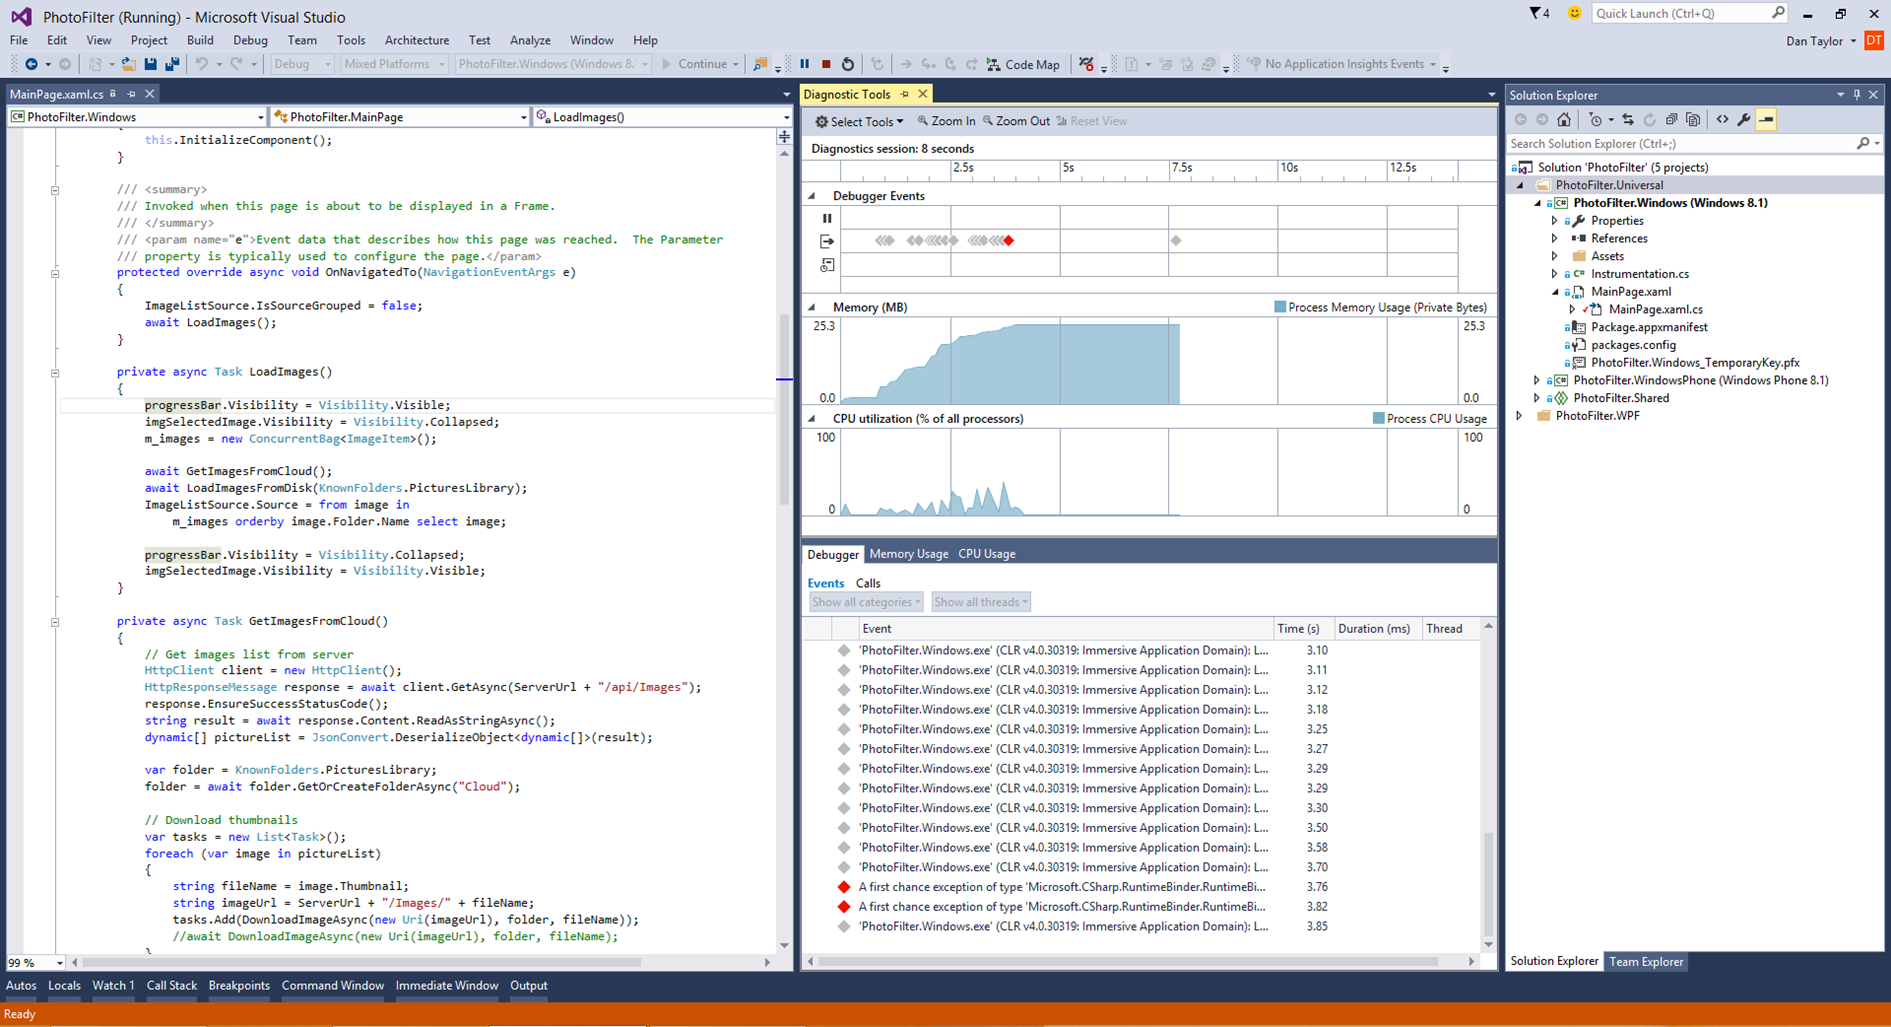
\includegraphics[width=0.9\linewidth]{images/dummy}
    \caption{some dummy}
\label{fig:dummy}
\end{figure}

\subsection{Ansible}
\label{sub:ansible}

\subsection{SaltStack}
\label{sub:saltstack}

\subsection{Packer}
\label{sub:packer}

\subsection{Habitat}
\label{sub:habitat}


\section{Kombinationsmöglichkeiten der Werkzeuge}
\label{sec:werkzeugkombinationsmoeglichkeiten}
